%Preamble

\documentclass{beamer}
\usepackage{pgf}
\usepackage{xcolor}
\usetheme{AnnArbor}
\usefonttheme{serif}

\usepackage{amssymb}
\usepackage{amsfonts}
\usepackage{amsmath}


\usepackage[bottom, hang, flushmargin]{footmisc}
\usepackage{indentfirst}
\usepackage{endnotes}
\usepackage{graphicx}
\usepackage{rotating}
\usepackage{natbib}
\usepackage{enumerate}
\usepackage{hyperref}
\usepackage{subfigure}
\usepackage{float}



\title{:-)}
\subtitle{}
\author{Da Hawk}
\date{\today} 


\AtBeginSection[]
{
  \begin{frame}
    \frametitle{Table of Contents}
    \tableofcontents[currentsection]
  \end{frame}
}

\begin{document}

\begin{frame} 
	\titlepage 
\end{frame}

\section{Graphs (1)}
\begin{frame}
	\frametitle{Monthly S\&P 500}
\begin{figure}[h]
	\begin{center}	
		\subfigure[Montly S\&P 500 Index]{
		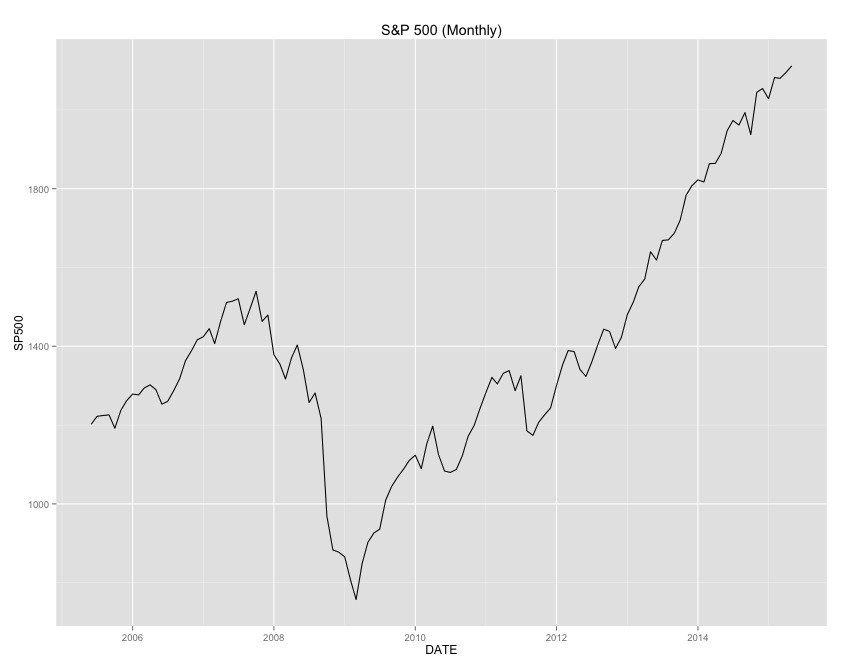
\includegraphics[scale=0.195]{sp500month.jpeg}}	
		\subfigure[Logged Montly S\&P 500 Index]{
		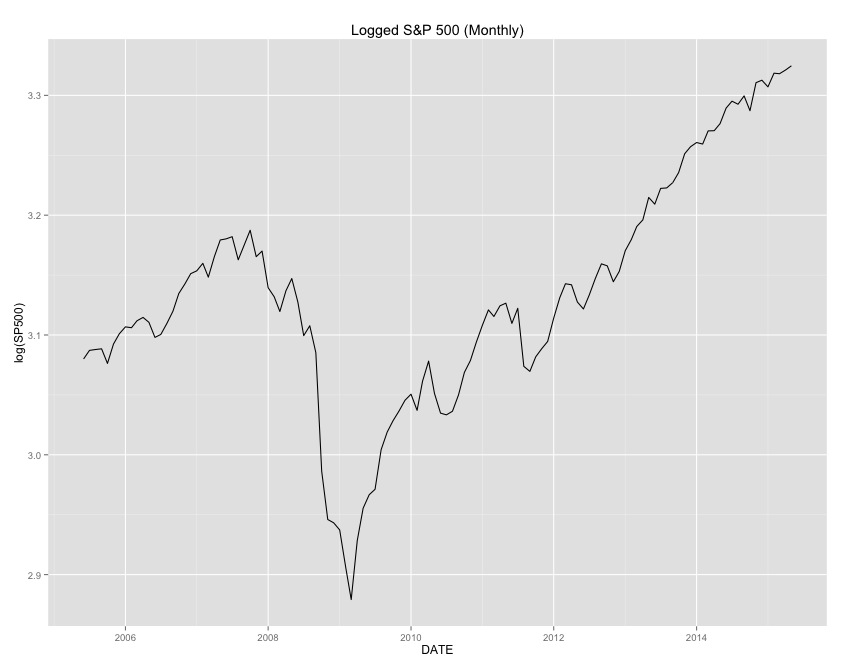
\includegraphics[scale=0.195]{logsp500month.jpeg}}
	\end{center}
\end{figure} 
\end{frame}


\begin{frame}
	\frametitle{Weekly S\&P 500}
\begin{figure}[h]
	\begin{center}	
		\subfigure[Weekly S\&P 500 Index]{
		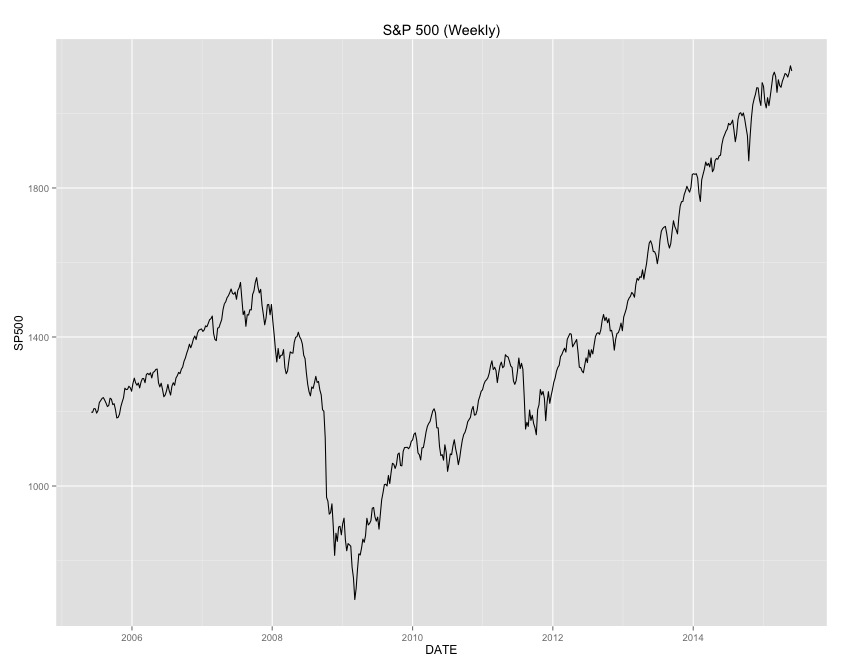
\includegraphics[scale=0.195]{sp500week.jpeg}}	
		\subfigure[Logged Weekly S\&P 500 Index]{
		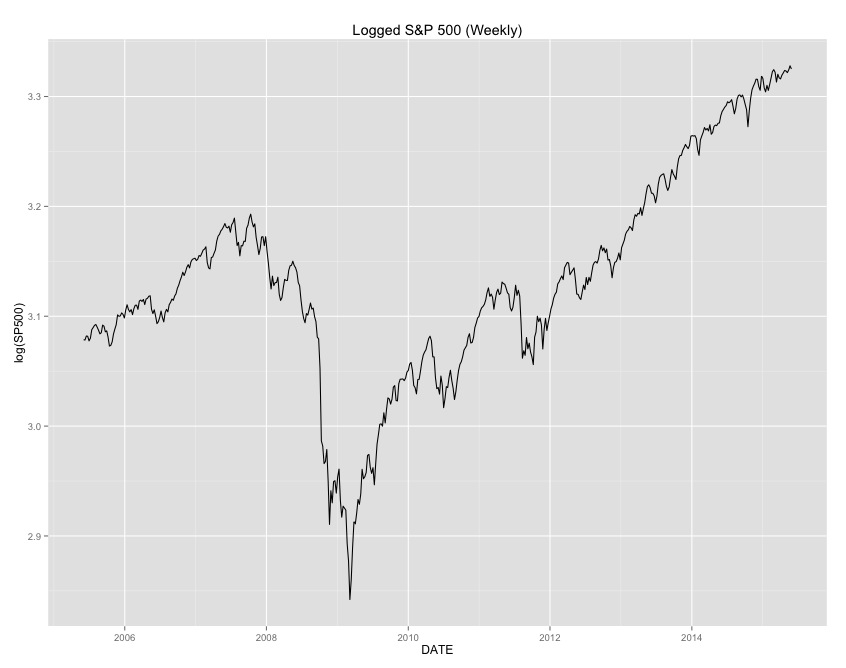
\includegraphics[scale=0.195]{logsp500week.jpeg}}
	\end{center}
\end{figure} 
\end{frame}

\section{Methods}
\begin{frame}
	\frametitle{Holt-Winters method}
Holt-Winters is an (triple) exponential smoother that decomposes a time series into three components
		\begin{itemize}
			\item Level
			\item Trend
			\item Seasonal
		\end{itemize}
Forecasts for the Monthly and Weekly S\&P 500 will be compared one-year out
		\begin{itemize}
			\item 52 weeks (weekly)
			\item 12 months (monthly)
		\end{itemize}
\end{frame}

\section{Tables}
\begin{frame}
	\frametitle{Tabels}
\begin{table}[H]
\center
\begin{tabular}{c c c c c}
\hline
Period & Forecast & Lo95 & Hi95 & Observed \\
\hline
51 & 2053.374 & 1699.511 & 2407.237 & 2127.95   \\
52 & 2045.534 & 1688.227 & 2402.841 & 2113.97  \\
\hline
11 & 2160.959 & 1623.475 & 2698.442 & 2094.86  \\
12 & 2157.658 & 1576.201 & 2739.114 & 2111.94  \\
\hline
\end{tabular}
\caption{Weekly v. Monthly Raw Forecaste}
\begin{tabular}{c c c c c}
\hline
Period & Forecast & Lo95 & Hi95 & Observed \\
\hline
51 & 3.330807 & 3.189547 & 3.472066 & 3.327961  \\
52 & 3.324947 & 3.182309 & 3.467584 & 3.325099  \\
\hline
11 & 3.351797 & 3.109288 & 3.594306 & 3.321155  \\
12 & 3.349269 & 3.083922 & 3.614616 & 3.324682  \\
\hline
\end{tabular}
\caption{Weekly v. Monthly Logged Forecaste}
\end{table}
\end{frame}


\section{Graphs (2)}
\begin{frame}
	\frametitle{Monthly S\&P 500 Forecast}
\begin{figure}[h]
	\begin{center}	
		\subfigure[Untransformed]{
		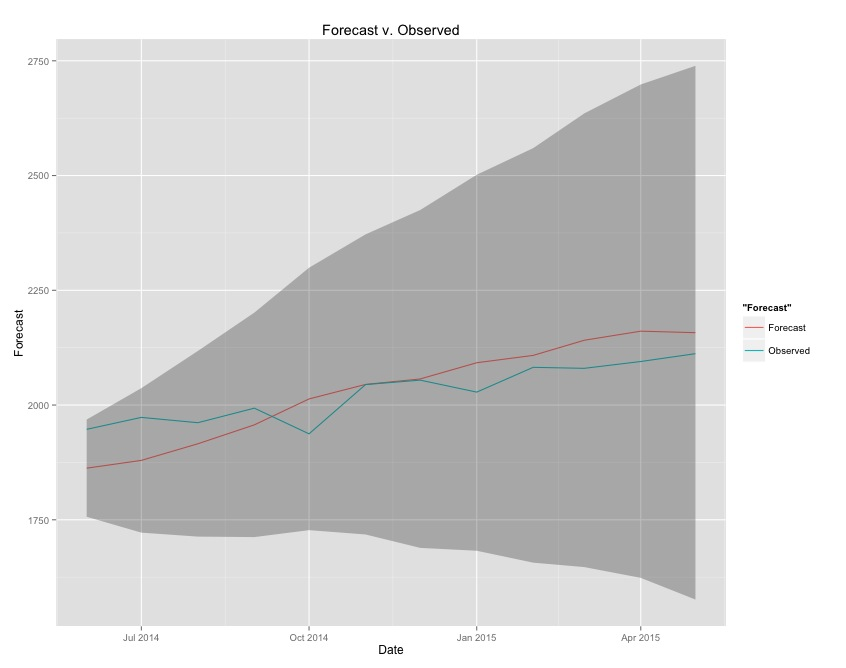
\includegraphics[scale=0.195]{month12.jpeg}}	
		\subfigure[Logged Tranformed]{
		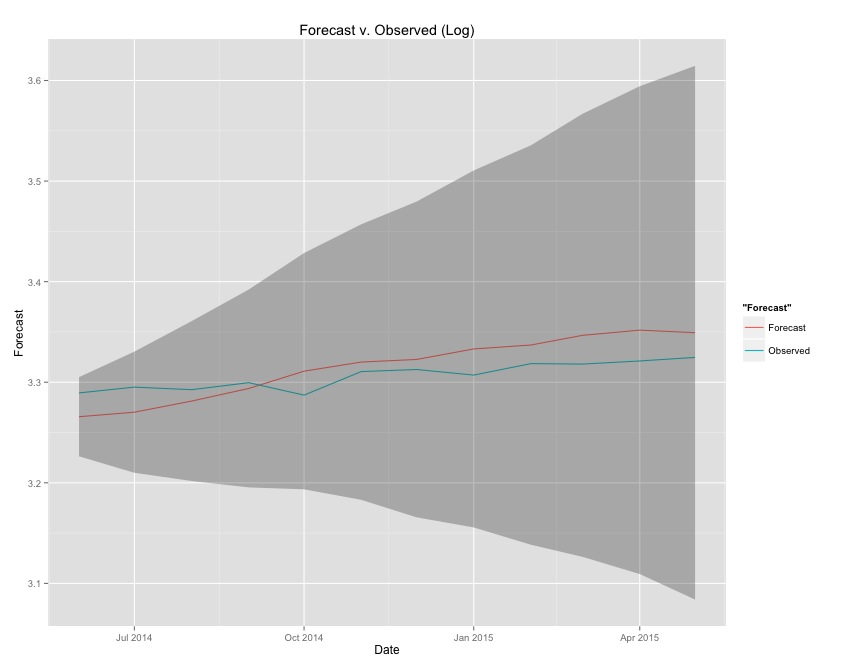
\includegraphics[scale=0.195]{logmonth12.jpeg}}
	\end{center}
\end{figure} 
\end{frame}


\begin{frame}
	\frametitle{Weekly S\&P 500 Forecast}
\begin{figure}[h]
	\begin{center}	
		\subfigure[Untransformed]{
		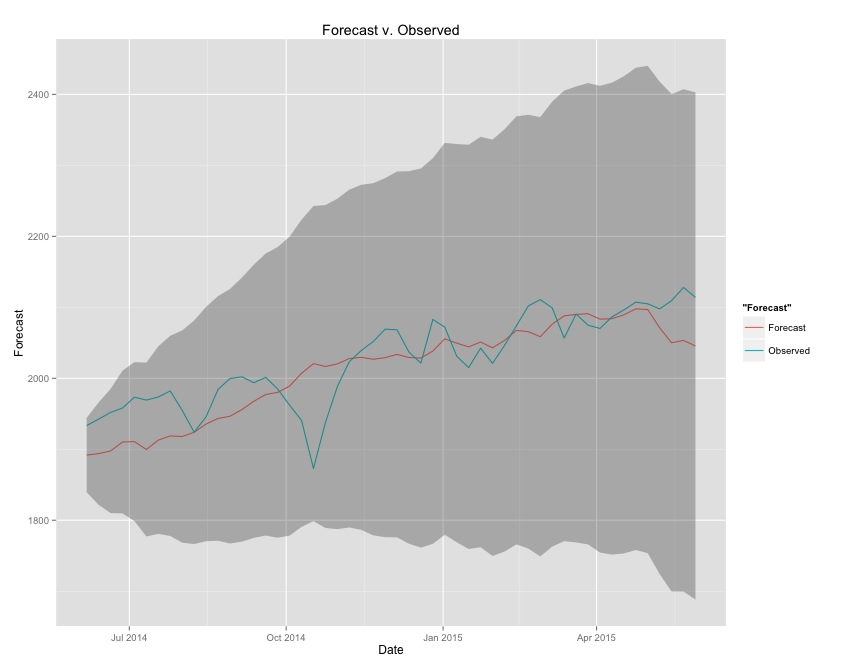
\includegraphics[scale=0.195]{week52.jpeg}}	
		\subfigure[Log Transformed]{
		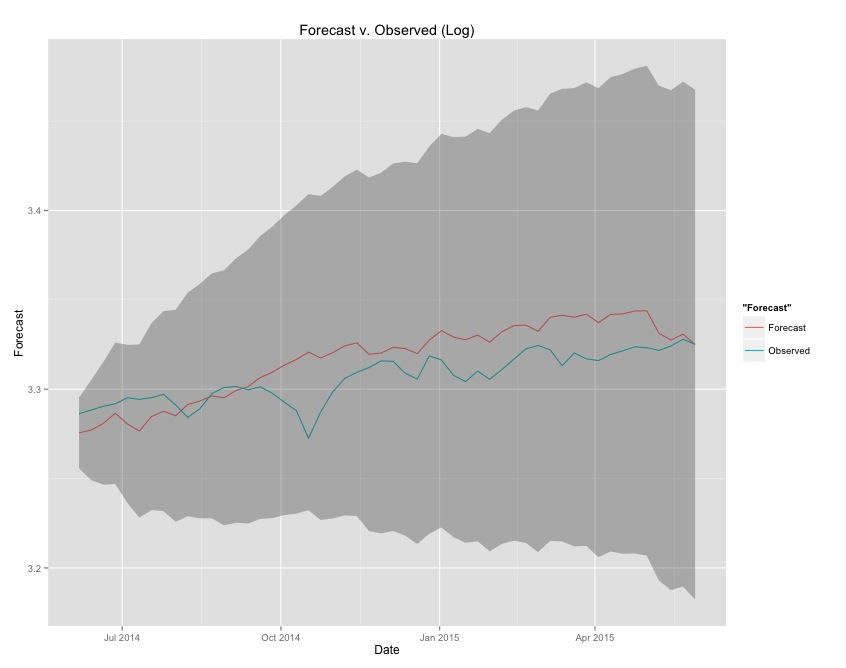
\includegraphics[scale=0.195]{weeklog52.jpeg}}
	\end{center}
\end{figure} 
\end{frame}

% etc
\end{document}

